\chapter{Prvá kapitola}
Skúšky najdôležitejších vecí.

\section{Matematika}
\[
u(x) =
  \begin{cases}
   \exp{x} & \text{if } x \geq 0 \\
   1       & \text{if } x < 0
  \end{cases}
\]

\section{Citácie}
Citovanie \citep{blackholes} zdroja.

\section{Obrázky}
Na obrázku \ref{fig:obrazok} vidieť autora \TeX-u ako sa učí používať \LaTeX.
\begin{figure}[h]
    \centering
    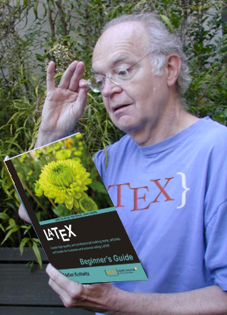
\includegraphics[width=0.5\textwidth]{knuth}
    \caption{Donald Knuth}
    \label{fig:obrazok}
\end{figure}
    
\section{Tabuľky}
Pomocka na Sudoku je v tabulke \ref{tab:numbers}.
\begin{center}
    \captionof{table}{Čísla od 1 po 9} \label{tab:numbers} 
    \begin{tabular}{l | c | r}
        1 & 2 & 3 \\ \hline
        4 & 5 & 6 \\ \hline
        7 & 8 & 9
    \end{tabular}
\end{center}

\section{Kód}
Ukážka nejakého kódu je v kóde \ref{lst:easter}.

\begin{listing}
\begin{minted}[mathescape,
               linenos,
               numbersep=5pt,
               frame=lines,
               framesep=2mm]{python3}
# V komentároch môže byť diakritika
# Alebo aj matika: $\lim_{x\to\infty}\exp(-x)=0$
import sys

str = sys.stdin.readline().strip()
if str.count('((') > 0:
    print('-1')
elif len(str) == 1:
    if str[0] == ')':
        print('0')
    else:
        print('-1')
elif str[-1:] == '(':
    print('-1')
else:
    print(str.count('('))               
\end{minted}
\caption{Veľkonočný zdroják}
\label{lst:easter}
\end{listing}

\section{Hlavička}
V hlavičke je kapitola a sekcia, ďalšie sekcie sú len na ukážku toho\footnote{Ukážka poznámky pod čiarou}.

\section{Lorem}
\lipsum[1]

\section{Ipsum}
\lipsum[2]